
\documentclass[extendedabs]{AAVL}

\runninghead{Claus, Fitzgibbon}{Plumbline Constraint for the RF Model}

\begin{document}

\title{Numerical simulations for selected 1D and 2D Mass-spring
models and Applications}

\addauthor{Sachin Chandrasekara}{SC/2018/10559}{1}


\addinstitution{
Department of Mathematics,\\
Faculty of Science,\\
University of Ruhuna}

\maketitle
\section{Problem statement}
\label{aa}

\noindent
A block is attached to the sides of a square box by 4 springs. The box is placed horizontally on a frictionless surface (ignore gravity). The mass of the block is m, the natural length of each spring is l, and the strength of each spring is k. Place the block at (0,0). Let $x(t),y(t)$ the position of the block in time. Find the equations of motion of the block.


\begin{figure}[hbt!]
\centering
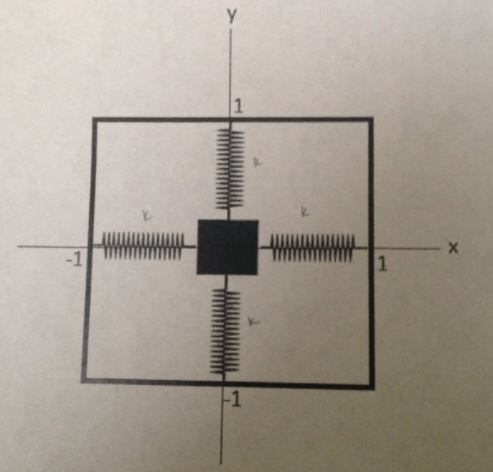
\includegraphics[width=6cm]{images/a.JPG}
\caption{2D spring mass system. }
\vspace{-2mm}
\label{fig:b}
\end{figure}

\section{Approach}
In this section, I have described some of the theories and assumptions I have already used. 


\begin{figure}[hbt!]
\centering
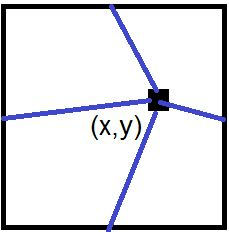
\includegraphics[width= 5cm]{images/b.JPG}
\caption{2D spring mass system. }
\vspace{-2mm}
\label{fig:b}
\end{figure}

You need the change of lengths of the springs when the block is removed from the central position. Each string is fixed to the middle point of the wall, so you need the distances of the block from these middle points. The forces act along the springs, break each force up the vertical and horizontal components. 

\subsection{The Euler-Lagrange equations}
\label{ab}
Here is the procedure. Consider the following seemingly silly combination of the kinetic and potential energies ($T$ and $V$ , respectively), It is denoted by $L$,
\begin{equation}
\label{1}
    L = T-V
\end{equation}

 The governing equations can also be achieved by following Lagrange's Equation directly. The expression for kinetic energy is,
\begin{equation}
\label{2}
    T = \frac{1}{2}m(\dot{x}^2 + \dot{y}^2)
\end{equation}
And also, the expression for potential energy is,

\begin{align}
\label{3}
\begin{split}
    V = \frac{1}{2}k(\sqrt{x^2+(y-l)^2}- l^2 )^2+ \frac{1}{2}k(\sqrt{(x+l)^2+y^2}- l^2 )^2 + \\ \frac{1}{2}k(\sqrt{x^2+(y+l)^2}- l^2 )^2   + \frac{1}{2}k(\sqrt{(x-l)^2+y^2}- l^2 )^2 
    \end{split}
\end{align}
Applying equations \eqref{2} and \eqref{3} to equation \eqref{1},
\begin{align}
\label{4}
    \begin{split}
        L = \frac{1}{2}m(\dot{x}^2 + \dot{y}^2) - \bigg ( \frac{1}{2}k(\sqrt{x^2+(y-l)^2}- l^2 )^2 + \\ \frac{1}{2}k(\sqrt{(x+l)^2+y^2}- l^2 )^2 + \\ \frac{1}{2}k(\sqrt{x^2+(y+l)^2}- l^2 )^2  + \\\frac{1}{2}k(\sqrt{(x-l)^2+y^2}- l^2 )^2 \bigg )
    \end{split}
\end{align}


Applying Lagrange’s equation to equation \eqref{4},
\begin{align}
\label{5}
\begin{split}
    \frac{d}{dt}(\frac{\partial L}{\partial \dot{x}})-\frac{\partial L}{\partial x} & = 0  \\
      m \Dot{x} - \bigg[ \dfrac{kx\left(\sqrt{x^2+\left(y-l\right)^2}-l^2\right)}{\sqrt{x^2+\left(y-l\right)^2}\\+ \dfrac{k\left(x+l\right)\left(\sqrt{\left(x+l\right)^2+y^2}-l^2\right)}{\sqrt{\left(x+l\right)^2+y^2}}
} \\ + \dfrac{kx\left(\sqrt{x^2+\left(y+l\right)^2}-l^2\right)}{\sqrt{x^2+\left(y+l\right)^2}} \\ + \dfrac{k\left(\sqrt{\left(x-l\right)^2+y^2}-l^2\right)^2}{2}
\bigg]& = 0   \\
    \end{split}
\end{align}

Applying Lagrange’s equation to equation \eqref{4},

\begin{align}
\label{6}
    \begin{split}
        \frac{d}{dt}(\frac{\partial L}{\partial \dot{x1}})-\frac{\partial L}{\partial x1} &= 0 \\
          m \Dot{y} - \bigg[ \dfrac{k\left(y-l\right)\left(\sqrt{\left(y-l\right)^2+x^2}-l^2\right)}{\sqrt{\left(y-l\right)^2+x^2}}\\ + \dfrac{ky\left(\sqrt{y^2+\left(x+l\right)^2}-l^2\right)}{\sqrt{y^2+\left(x+l\right)^2}}\\+ \dfrac{k\left(y+l\right)\left(\sqrt{\left(y+l\right)^2+x^2}-l^2\right)}{\sqrt{\left(y+l\right)^2+x^2}}\\+ \dfrac{ky\left(\sqrt{y^2+\left(x-l\right)^2}-l^2\right)}{\sqrt{y^2+\left(x-l\right)^2}}
\bigg]& = 0   \\
    \end{split}
\end{align}




 
  


\end{document}
